\section{Evaluation}
\label{sec:eval}


\subsection{Experimental Setup}
\label{subsec:eval_setup}

\begin{figure*}
    \centering
    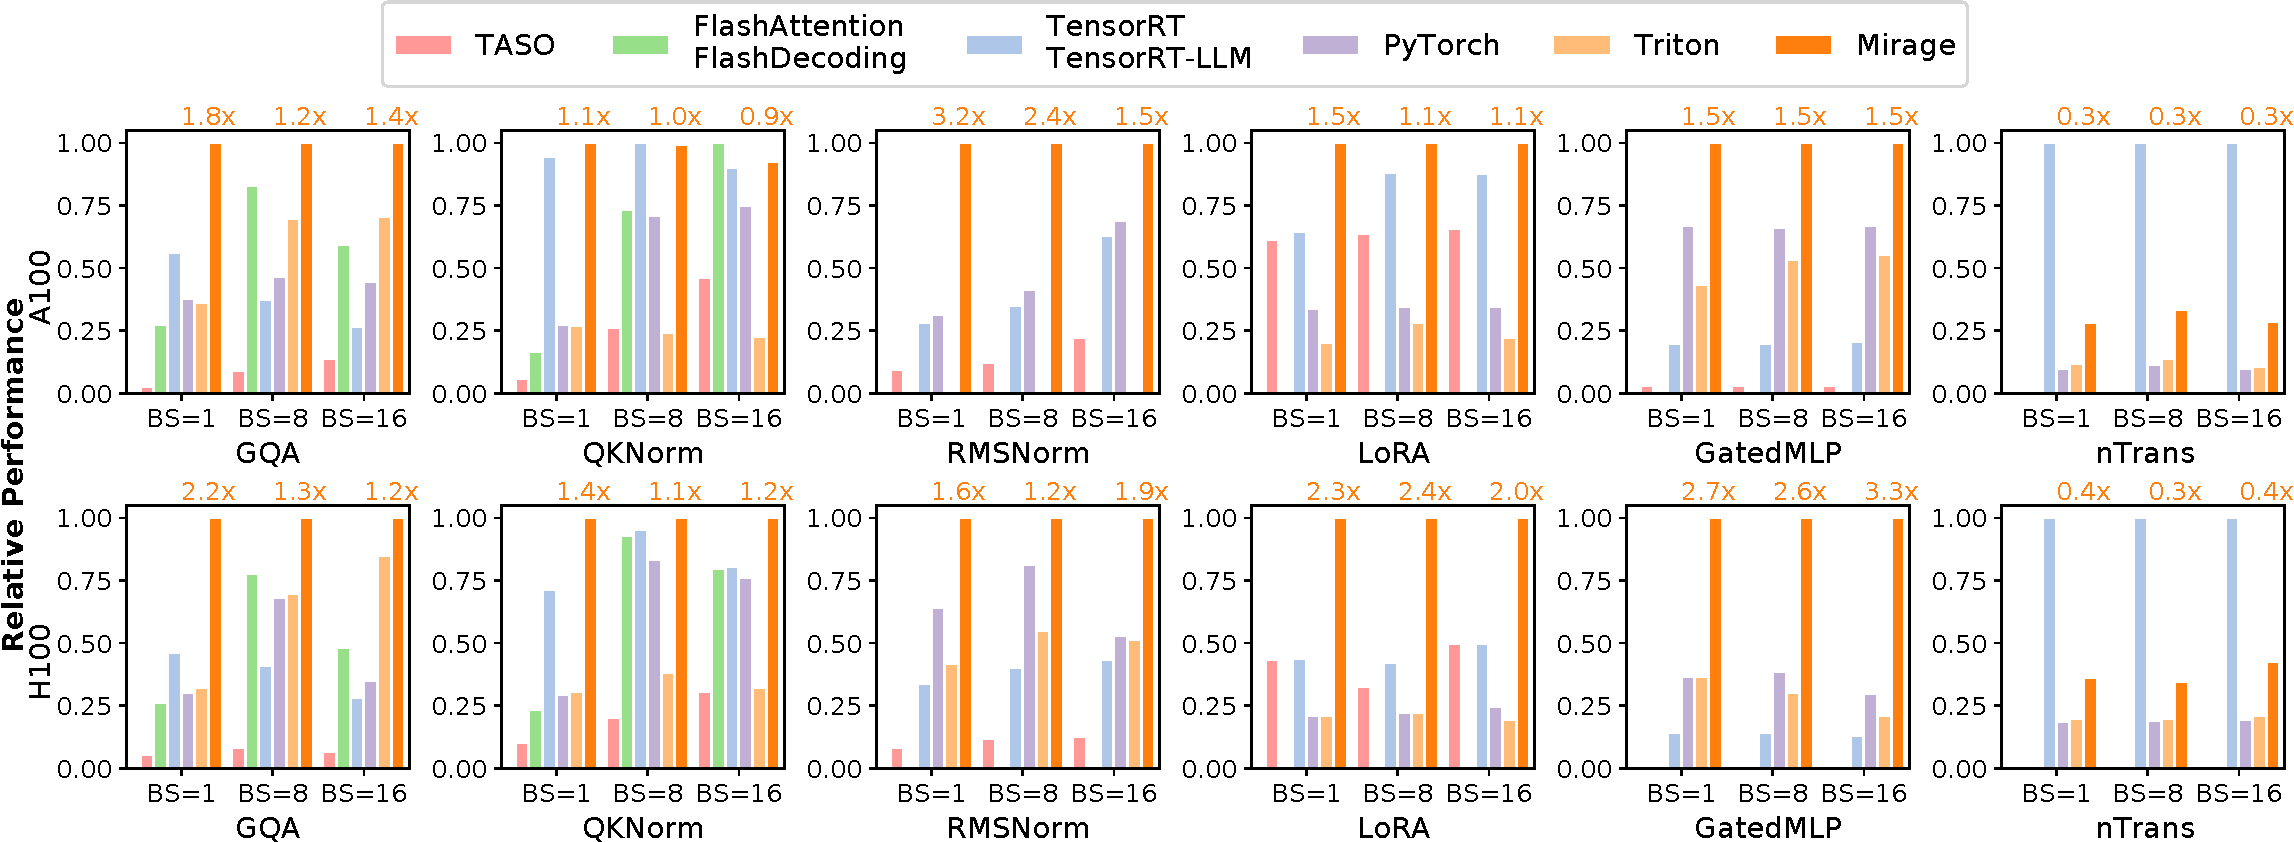
\includegraphics[width=\textwidth]{figs/benchmark-crop.pdf}
    \vspace{-1em}
    \caption{Comparing \sys with existing systems for 6 benchmarks on an A100 and an H100 GPU. The performance of all systems are normalized by \sys (higher is better). Numbers above the \sys bars show the speedup over the best baselines.}
    \vspace{\captionvspace}
    \label{fig:benchmarks}
\end{figure*}

\if 0
\begin{table}
    \centering
    \caption{DNN benchmarks used in our evaluation.}
    \vspace{\captionvspace}
    \footnotesize
    \label{tab:benchmarks}
    \begin{tabular}{l|l|l}
    \toprule
    {\bf Name} & {\bf Description} & {\bf Base Architecture} \\
    \midrule
    MHA & Multi-head attention (3 modes) & \llama-7B~\cite{touvron2023llama}\\
    GQA & Group-query attention (3 modes) & \llama-2-70B~\cite{llama2} \\
    MQA & Multi-query attention (3 modes) & Falcon-7B~\cite{falcon40b} \\
    MLP & Multi-layer perceptron & Adapter Tuning~\cite{houlsby2019parameter} \\
    MoE & Mixture-of-experts & Mixtral-7B~\cite{jiang2023mistral} \\
    LoRA & Low-rank adaptation & \llama-7B-LoRA~\cite{llama-7b-lora} \\
    \bottomrule
    \end{tabular}
    \vspace{\captionvspace}
\end{table}
\fi 

Since \sys is a superoptimizer for \lax programs, we focus our evaluation on various DNN benchmarks commonly used in existing DNNs, each of which is a \lax program.
These benchmarks provide the most fine-grained way to compare the performance of \sys and existing systems.
\Cref{tab:benchmarks} shows the six benchmarks in our evaluation.
%including (1) multi-head attention (MHA), (2) group-query attention (GQA), (3) multi-query attention (MQA), (4) multi-layer perception (MLP), (5) mixture-of-experts (MoE), and (6) low-rank adapters (LoRA).
GQA, RMSNorm, and GatedMLP are the main building blocks of large language models (LLMs).
%
%GQA and MQA reduce memory requirements of MHA and have been widely deployed in recent LLMs. 
QKNorm introduces query-key normalization before attention to enhance model convergence~\cite{chameleonteam2024chameleon}.
%MoE uses multiple experts, each of which is an MLP architecture, to improve the predictive performance of a DNN without increasing its latency.
LoRA enables low-rank adaptation for fine-tuning a DNN on different tasks.
We use a context length of 8K for GQA and 4K for QKNorm, corresponding to the maximum supported by \llama-3-70B~\cite{grattafiori2024llama3herdmodels} and Chameleon-7B~\cite{chameleonteam2024chameleon}, respectively.
In addition, we also evaluate how \sys-generated kernels improve the end-to-end performance of full DNNs, including Chameleon~\cite{chameleonteam2024chameleon}, nGPT~\cite{loshchilov2024ngpt}, \llama-3~\cite{grattafiori2024llama3herdmodels}, and LoRA~\cite{hu2021lora}.

%
%For all attention mechanisms, we assume 4096 key-value tokens and evaluate \sys in three different scenarios: incremental decoding (1 query token), speculative decoding (32 query tokens), and chunked pre-filling (512 query tokens).
%\oded{are those three scenarios reflected in \Cref{fig:benchmarks}? Do we report the mean over the three scenarios?}
%

%We use a Perlmutter compute node for all experiments~\cite{perlmutter}, which is equipped with four NVIDIA 40GB A100 GPUs and 256 GB DRAM.
%
The experiments were conducted on NVIDIA A100 and H100 GPUs, each with 40GB of memory.
All our benchmarks fit on a single GPU except GQA (used for \llama-2-70B), which is generally parallelized across four GPUs using tensor model parallelism~\cite{Megatron}.
%
Therefore, we evaluate GQA under this parallelism strategy, where the eight key-value heads are equally partitioned across four GPUs.
Since the performance of \sys and all baselines depends only on the shapes of the input tensors, we repeat each experiment 1,000 times using random inputs and report the average run time. %We observed negligible variance across different runs.
%\oded{why repeat 1000 times then?}

One of our benchmarks, LoRA, requires  concatenation to express a common optimization: fusing two matrix multiplications via concatenation. To support this optimization in \sys, we introduce a new linear operator that takes four inputs and computes $f(W, X, Y, Z) = (W \| X) \times (Y \| Z)$, where $\|$ is tensor concatenation.
This operator is equivalent to computing $W \times Y + X \times Z$.
We define the abstract expression associated with this operator as: 
$\expr(f(W, X, Y, Z)) = \eadd(\ered(k_1, \emul(\expr(W), \expr(Y))), \ered(k_2, \emul(\expr(X), \expr(Z))))$, where $k_1$ and $k_2$ are the last dimensions of $W$ and $X$.

Unless otherwise stated, \sys considers up to 5 operators in the kernel graph and up to 11 operators in each block graph.

%Note that the \sys \graph generator can discover \graphs for MLP, which is not a \lax tensor program due to {\tt ReLU}. The equivalence verifier cannot provide probabilistic correctness guarantees on non-\lax \graphs, which are manually verified in our evaluation. 
%\oded{This needs further explanation. What about the abstract expressions for Relu? Do we turn off pruning here? Without the verifier, wha bt even causes \sys to output a correct \graph? Do we also test using floating point? We should explain if so.}


\subsection{Benchmark Results}
\label{subsec:benchmark_results}
%\oded{I'd rename the subsection to: Performance Results}
\Cref{fig:benchmarks} compares the performance of \sys with systems on six DNN benchmarks on NVIDIA A100 and H100 GPUs.
All systems use half-precision floating points to run these DNN benchmarks.
%
TASO~\cite{TASO} and PET~\cite{wang2021pet} are DNN superoptimizers that automatically generate algebraic transformations at the kernel level.
We report a combined TASO/PET baseline, as the latest TASO implementation includes PET’s partially equivalent transformations as special substitutions.
%
PyTorch~\cite{pytorch} uses the highly optimized cuDNN and cuBLAS libraries~\cite{cublas,cudnn} to perform DNN operators on GPUs.
For the PyTorch baseline, we enable {\tt torch.compile} and use FlashAttention kernels to maximize performance.
%
TensorRT and its LLM variant TensorRT-LLM include a set of manually designed and highly optimized kernels for common tensor operators such as attention~\cite{tensorrt}.
%
FlashAttention and its inference variant FlashDecoding are manually written kernels for efficient attention~\cite{dao2023flash, hong2024flashdecoding}.
Finally, Triton is a schedule-based optimizer to generate high-performance kernels and has been adopted in production systems, outperforming other schedule-based approaches~\cite{tillet2019triton}.
All baselines use CUDA Graphs to minimize kernel launch overhead.
%
%We do not compare \sys with existing superoptimizers (e.g., TASO~\cite{TASO} or PET~\cite{wang2021pet}) since the DNNs we use as input do not contain purely algebraic optimization opportunities at the kernel level.
%are already in their optimal forms, so these superoptimizers cannot further improve performance.
%\oded{are we sure? how come?}

%\oded{shouldn't we refer to \Cref{fig:benchmarks} here? Maybe update the opening sentence above to:
%\Cref{fig:benchmarks} compares ...}
%\oded{what's the BS=1 BS=8 in the figure? I think we never explain it}

Compared to the best existing approaches, \sys improves the performance of these benchmarks by up to $3.3\times$ by combing algebraic transformations, schedule transformations, and the generation of new custom kernels. \S\ref{sec:case2} shows the best discovered \graphs for RMSNorm. Next, we present a case study for the remaining benchmarks.

\begin{figure}
    \centering
    \subfloat[The kernel graph for QKNorm and attention in existing systems.]{
    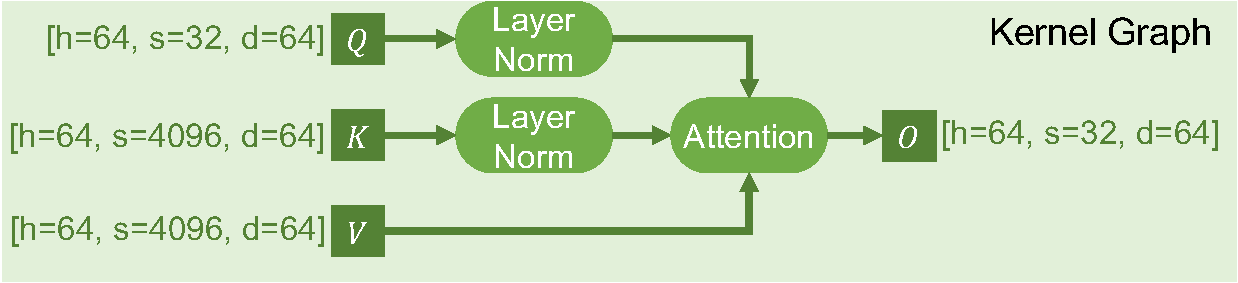
\includegraphics[scale=0.37]{figs/qknorm_attn_baseline-crop.pdf}
    \label{fig:qknorm_baseline}
    }
    \\
    \subfloat[The best \graph discovered by \sys for QKNorm and attention.]{
    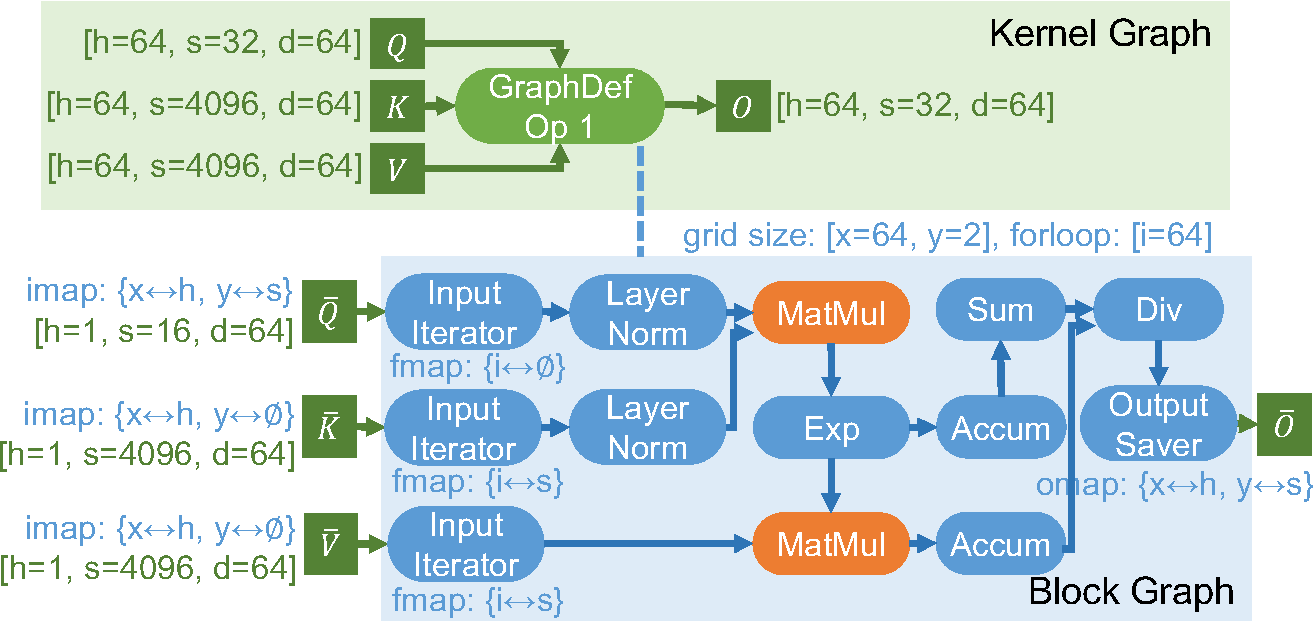
\includegraphics[scale=0.37]{figs/qknorm_attn_ours-crop.pdf}
    \label{fig:qknorm_ours}
    }
    \vspace{\captionvspace}
    \caption{Comparing the \graphs used by existing optimizers and \sys for QKNorm and attention.}
    \vspace{\captionvspace}
    \label{fig:qknorm_example}
\end{figure}

\paragraph{GQA.} Group-query attention is the backbone of LLMs and has been heavily optimized by existing frameworks. For example, FlashAttention and FlashDecoding are expert-designed attention kernels and have been adopted in existing LLM inference systems~\cite{dao2023flash}.
%
\sys discovers these expert-designed kernels as well as other \graphs that outperform them by up to 2.2$\times$.
The speedup is achieved by two additional optimizations on top of existing hand-written kernels. First, current approaches rely on fixed heuristics to determine the grid dimensions for GQA, which are suboptimal in certain scenarios. For example, TensorRT-LLM launches the GQA kernel with grid dimensions of (8, 2, 1) and (8, 2, 8) when the batch sizes are 1 and 8, respectively. However, both configurations cannot fully utilize all SMs on A100 (108 SMs) and H100 (132 SMs) GPUs. 
In contrast, \sys automatically searches for the best grid dimensions for each \graph, resulting in full SM utilization.
Further ablation study shows that the performance of the best \graph discovered by \sys degrades by 18\% when using the same grid dimensions as TensorRT-LLM.

Second, existing approaches use fixed tensor dimensions to parallelize GQA across thread blocks. For example, FlashAttention~\cite{dao2023flash} parallelizes attention across the {\em sample}, {\em head}, and {\em query sequence} dimensions, while FlashDecoding and TensorRT-LLM leverage the {\em sample}, {\em head}, and {\em key-value sequence} dimensions. Both strategies are efficient for conventional multi-head attention with many heads but suboptimal for GQA with fewer attention heads.
In contrast, \sys automatically selects the most efficient parallelization strategy by choosing among the sample, KV heads, query sequence, and key-value sequence dimensions. Moreover, \sys generates different \graphs tailored to different attention scenarios, reducing device memory access by up to 7$\times$ compared to the heuristics used in existing systems.
%
%\Cref{fig:gqa_comparison} compares the FlashAttention kernel and \sys's generated kernel for GQA in the single-batch speculative decoding phase.
%
%Instead of parallelizing across the sample, head, and query sequence dimensions, \sys finds a \graph that parallelizes across the head, query sequence, and key-value sequence dimensions. As a result, each block only needs to load 256/8=32 query vectors, 1024/8=128 key vectors, and 1024/8=128 value vectors, reducing memory access by 7$\times$ and kernel execution time by 2.2$\times$.

Implementing \sys's \graphs in existing systems is possible but requires extensive engineering effort to support different kernels for different scenarios. In contrast, \sys automatically generates them and verify their correctness.

\paragraph{QKNorm.} To reduce model divergence, several recent DNNs introduce query-key normalization (QKNorm) into the Transformer architecture~\cite{chameleonteam2024chameleon}. QKNorm applies layer normalization to the query and key vectors before attention, as shown in \Cref{fig:qknorm_baseline}. These additional normalization layers are not yet supported by existing attention implementations (e.g., FlashAttention and TensorRT-LLM) and require launching separate kernels for normalization and attention.

\Sys automatically discovers a \graph that integrates QKNorm and attention computation into a custom kernel, as shown in \Cref{fig:qknorm_ours}. The \graph reorganizes the attention computation to enable fusion with the two layer normalizations, which avoids writing intermediate results to GPU device memory and reduces the kernel execution time by up to 1.4$\times$.

\begin{figure}
    \centering
    \subfloat[The kernel graph for LoRA in existing systems.]{
    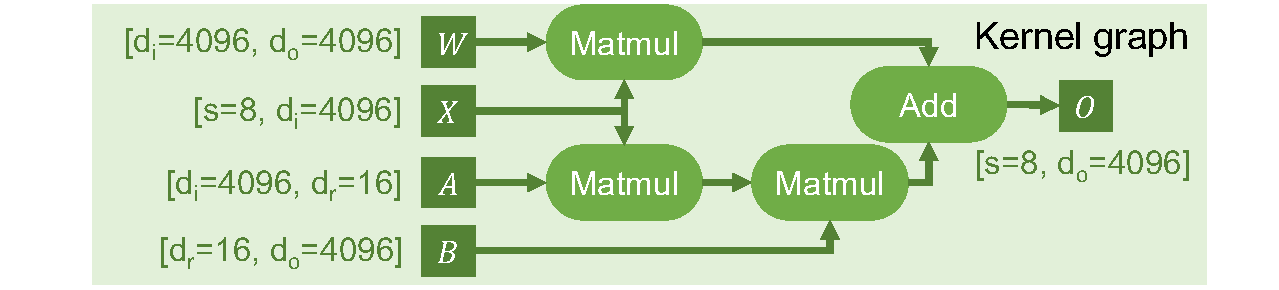
\includegraphics[scale=0.38]{figs/lora_baseline.pdf}
    \label{fig:lora_baseline}
    }
    \\
    \subfloat[The best \graph discovered by \sys for LoRA.]{
    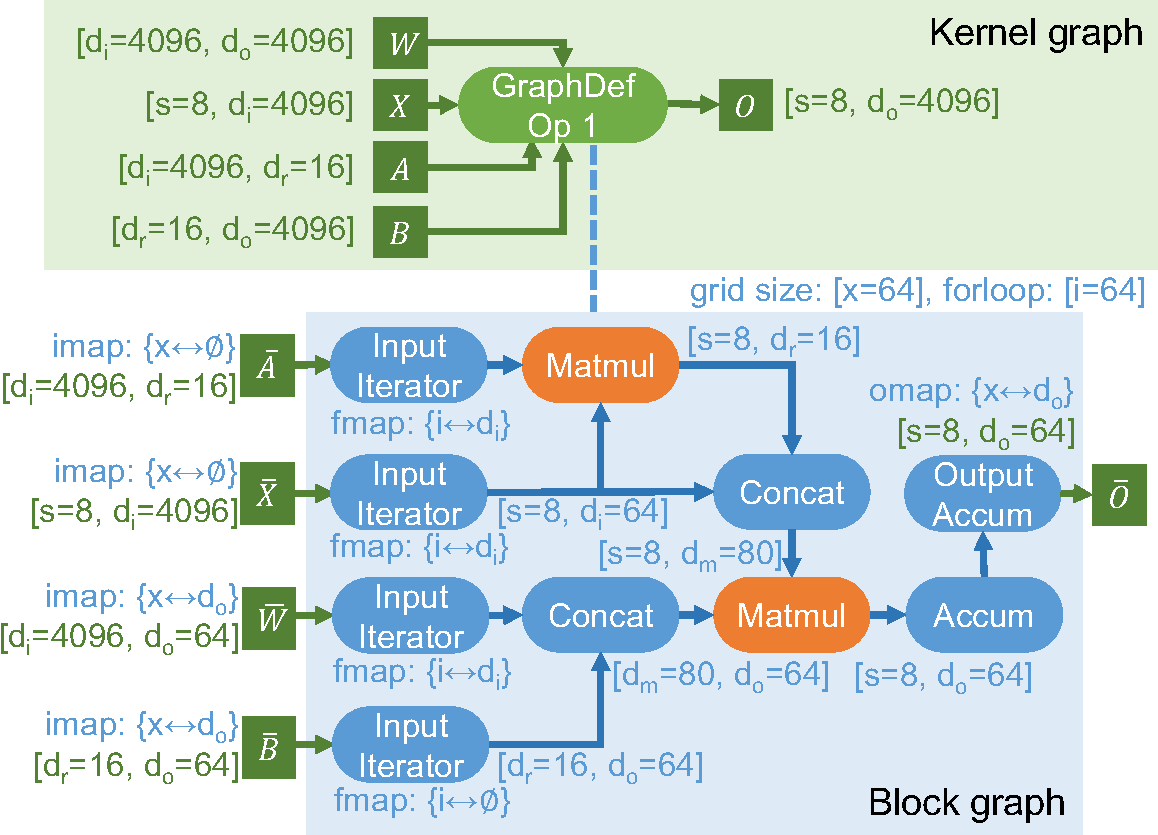
\includegraphics[scale=0.38]{figs/lora_ours_v2-crop.pdf}
    \label{fig:lora_ours}
    }
    \vspace{\captionvspace}
    \caption{Comparing the tensor programs used by existing optimizers and by \sys for LoRA: $O = W \times X + B \times A \times X$. Note that both matrices $A$ and $B$ are low-rank.}
    \vspace{\captionvspace}
    \label{fig:lora_example}
\end{figure}

\paragraph{LoRA.}
Low-rank adaptation (LoRA) introduces a pair of low-rank adapters to the linear operators of a pre-trained DNN to improve its performance for downstream tasks. 
%
Existing tensor program optimizers launch separate kernels for the original linear operator and the two additional linear operators introduced by LoRA (\Cref{fig:lora_baseline}), which introduces high kernel launch overheads since these LoRA operators involve minimal computation.
%
\Cref{fig:lora_ours} shows the best \graph discovered by \sys for LoRA, which fuses the three {\tt Matmul}s and the subsequent {\tt Add} into a single kernel. \sys reorganizes the computation into two block-level {\tt Matmul}s by leveraging the following algebraic transformation: $W \times X + B \times A \times X = (W \| B) \times \big(X \| (A\times X)\big)$. The {\tt Concat}s in \Cref{fig:lora_ours} do not involve any computation and are performed by updating tensor offsets in GPU shared memory.
%
This \graph reduces the execution cost of LoRA by
1.1-2.4$\times$.

\begin{figure}
    \centering
    \subfloat[The kernel graph for GatedMLP.]{
    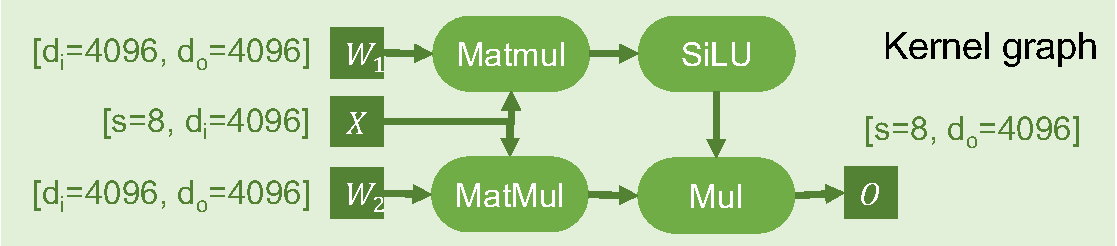
\includegraphics[scale=0.4]{figs/gated_mlp_baseline-crop.pdf}
    \label{fig:mlp_baseline}
    }
    \\
    \subfloat[The best \graph discovered by \sys for GatedMLP.]{
    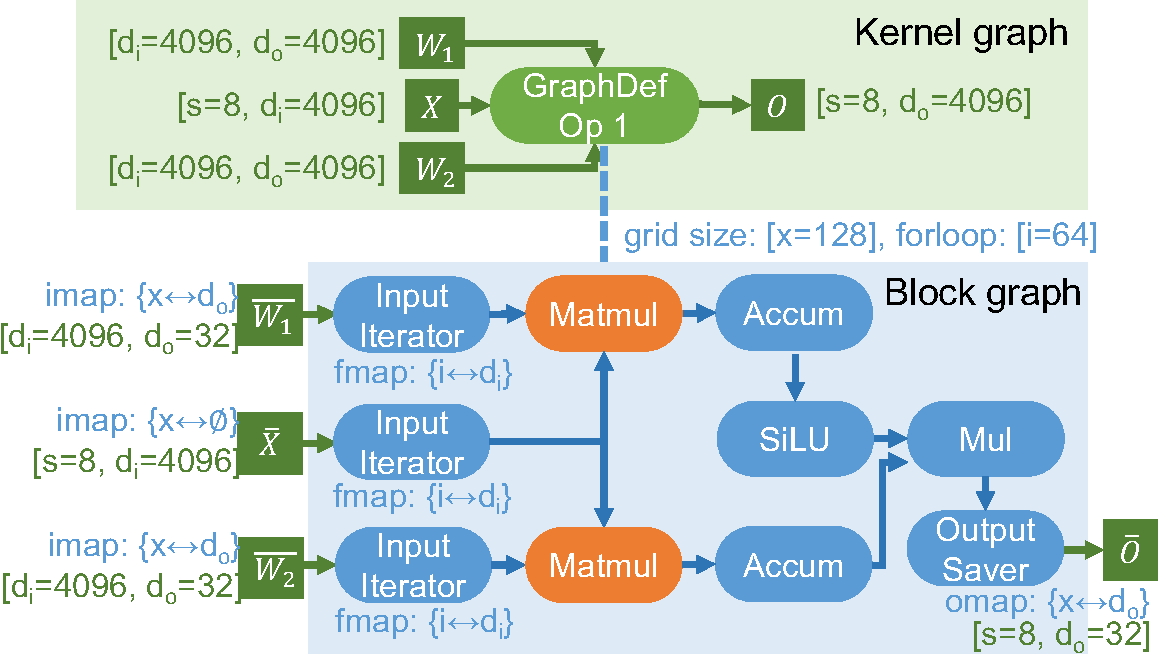
\includegraphics[scale=0.4]{figs/gated_mlp_ours-crop.pdf}
    \label{fig:mlp_ours}
    }
    \vspace{\captionvspace}
    \caption{Comparing the \graphs used by existing optimizers and \sys for GatedMLP.}
    \vspace{\captionvspace}
    \label{fig:mlp_example}
\end{figure}

\paragraph{GatedMLP.}
Gated multi-layer perceptrons are commonly used in DNNs to capture non-linear representations.
%
We use the GatedMLP configuration introduced in Falcon-7B~\cite{falcon40b}, whose kernel graph is shown in \Cref{fig:mlp_baseline}.
Existing tensor program optimizers generally fuse the two {\tt Matmul}s in a single kernel to reduce GPU device memory access, since the input tensor $X$ only needs to be loaded once.
%
However, this approach still requires launching multiple kernels and storing intermediate results---specifically, the output of the two {\tt Matmul}s---in device memory, as the {\tt SiLU} activation and elementwise multiplication are not fused with the {\tt Matmul}s. 
%

In contrast, the best \graph discovered by \sys (\Cref{fig:mlp_ours}) performs the two {\tt Matmul}s in parallel within the same block graph and fuses the remaining computation (i.e., {\tt SiLU} and {\tt Mul}) as post-processing steps within the same block graph. This approach yields 1.5$\times$ speedups on A100 GPUs and 2.7-3.3$\times$ speedups on H100 GPUs.

%In contrast, the best \graph discovered by \sys (\Cref{fig:mlp_ours}) performs {\em partial summation} of the first {\tt Matmul} in the first kernel, and fuses the remaining summation, {\tt ReLU}, second {\tt Matmul}, and {\tt Add} in the second kernel. 
%\MW{The second kernel is not shown in the figure. We need to explain, or it would be confusing.} 
%This design enables more parallelism for the first kernel and better utilizes an A100 GPU, yielding a 3$\times$ speedup.
%

\paragraph{nTrans.}
To accelerate model training, nGPT introduces normalized Transformer, which normalizes all intermediate results in Transformer~\cite{loshchilov2024ngpt}. Formally, the computation is defined as $y = \texttt{Norm}(x + \alpha (\texttt{Norm}(h - x)))$, where {\tt Norm} is a normalization layer, and $x$, $h$, and $\alpha$ are input tensors. Existing systems launch three separate kernels for nTrans, since it interleaves normalization and elementwise addition and multiplication. \Sys automatically discovers a \graph that fuses the computation into a single kernel and stores all intermediate results in GPU shared memory. \Sys outperforms other baselines but is slower than TensorRT. This performance gap is because \Sys loads data from global memory to shared memory and writes it back for each tensor in graph-defined kernels. This design improves memory efficiency and enables asynchronous pipelines. However, for kernels with light computation, the overhead of these memory transfers can dominate the kernel runtime. 
%which increases the kernel execution time by 1.8-2.0$\times$ compared to the best existing systems. 
To mitigate this overhead, we plan to extend \sys to support bypassing shared memory during data loading, therefore avoiding unnecessary data movement.

\begin{figure}
    \centering
    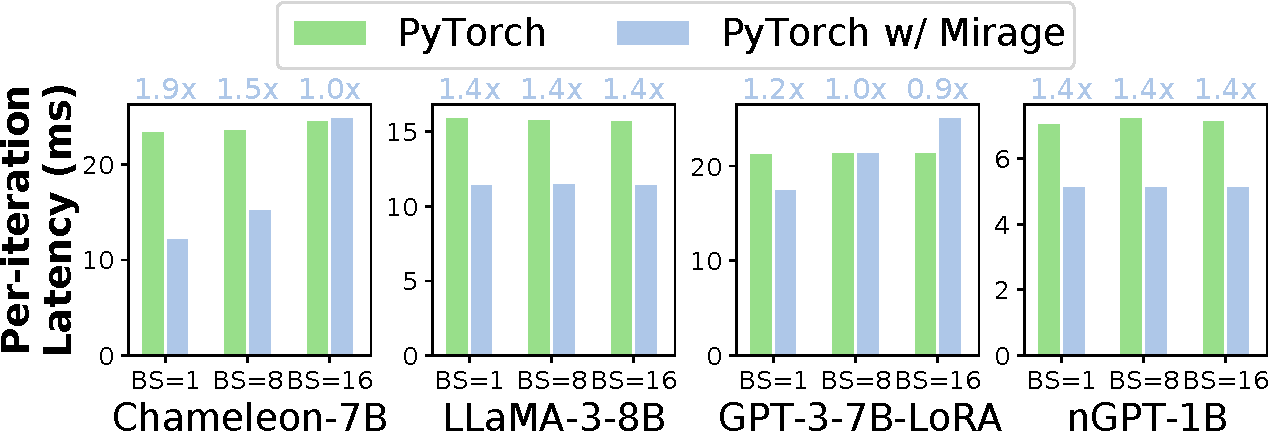
\includegraphics[width=\columnwidth]{figs/end2end-crop.pdf}
    \caption{Comparing the end-to-end inference performance of PyTorch and PyTorch with \sys-generated kernels.}
    \label{fig:end_to_end_models}
\end{figure}


\subsection{End-to-end Results}
In addition to the microbenchmark performance, we also evaluate how \sys-generated kernels impact the end-to-end latency of commonly used DNNs. \sys supports just-in-time compilation and deployment, and its generated kernels can be directly integrated into PyTorch programs. We compare PyTorch with its native handwritten CUDA kernels and PyTorch with \sys-generated kernels on four DNN models. \Cref{fig:end_to_end_models} shows the results. \sys reduces the end-to-end latency of these models by 0.9-1.9$\times$ by automatically generating highly optimized kernels. The improvement is achieved with a few lines of code changes to the PyTorch programs.

\subsection{Search Time}

\begin{table}
    \centering
    %\caption{Time for the \graph generator to generate all the \graphs for GQA (batch size 1) with up to a certain number of operators per block graph.}
    \caption{Ablation study on \sys's techniques to accelerate \graph generation. We evaluate the impact of multi-threading and abstract expressions on search time for RMSNorm.}
    \vspace{\captionvspace}
    \footnotesize
    \label{tab:search_time}
    \begin{tabular}{c|r|r|r}
    \toprule
    {\bf Max \# Ops in} & {\bf \sys} & {\bf \sys w/o } & {\bf \sys w/o }\\
    {\bf a Block Graph} & {\bf } & {\bf Multithreading} & {\bf Abstract Expression} \\
    \midrule
    $5$ & $11$ sec &$58$ sec  & $768$ sec \\
    $6$ & $16$ sec & $93$ sec & $19934$ sec \\
    $7$ & $22$ sec & $150$ sec & $> 10$ h \\
    $8$ & $24$ sec & $152$ sec & $> 10$ h \\
    $9$ & $26$ sec & $166$ sec & $> 10$ h \\
    $10$ & $26$ sec & $166$ sec & $> 10$ h \\
    $11$ & $28$ sec & $183$ sec & $> 10$ h \\
    \bottomrule
    \end{tabular}
    \vspace{\captionvspace}
\end{table}

In our evaluation, \sys takes up to 4 hours to optimize a \lax program. This optimization is a one-time cost before deployment on the target hardware.
This subsection provides detailed results and an ablation study of \sys's search procedure, focusing on how its techniques enable the exploration of large \graphs while maintaining low search time.
%
In particular, we evaluate the impact of two techniques: pruning via abstract expressions (\S\ref{subsec:abstract_expression}) and multi-threading.
%
\Cref{tab:search_time} reports the search times for RMSNorm as we vary the maximum number of operators allowed in a block graph.
% For searches that consider 4 operators in a block graph,
% pruning via abstract expressions slightly increases the search time due to the cost of SMT queries.
% For larger-scale searches, the pruning allows \sys to explore \graphs whose block graphs can each have at most 11 operators, while disabling abstract expression (and canonical form of \graphs) restricts \sys to consider up to 5 (and 4) operators in a block graph in order to finish the search in 12 hours. \MW{TBD}

Multi-threading significantly reduces the search time, while pruning via abstract expressions is crucial for the scalability of \sys.
%
Specifically, the pruning techniques allow \sys to explore \graphs whose block graphs can each have at most 11 operators, while disabling abstract expression pruning restricts \sys to handle block graphs with up to 6 operators within a 10-hour search window.
%
Note that discovering the optimized \graph for RMSNorm shown in \Cref{fig:mugraph} requires exploring block graphs with 11 operators.


\if 0
\begin{table}
    \centering
    %\caption{Time for the \graph generator to generate all the \graphs for GQA (batch size 1) with up to a certain number of operators per block graph.}
    \caption{Ablation study on \sys's techniques to accelerate \graph generation. We incrementally disable abstract expression (\S\ref{subsec:abstract_expression}) and canonical form (\S\ref{subsec:kernel_block_graph_generation}), then evaluate the search times as we adjust the maximum number of operators within a block graph.}
    \vspace{\captionvspace}
    \small
    \label{tab:search_time}
    \begin{tabular}{c|r|r|r}
    \toprule
    {\bf \# Ops per} & {\bf MISO} & {\bf MISO w/ redundancy} & {\bf MISO}\\
    {\bf Kernel} & {\bf w/o Opt} & {\bf  pruning only} & {\bf }\\
    \midrule
    $2$ & $< 1$sec & $< 1$sec & $3$sec \\
    $3$ & $< 1$sec & $< 1$sec & $3$sec \\
    $4$ & $< 1$sec & $< 1$sec & $9$sec \\
    $5$ & $> 12$h & $249$ min & $2.3$ min \\
    $6$ & $> 12$h & $> 12$h & $20$ min \\
    $7$ & $> 12$h & $> 12$h & $76$ min \\
    \bottomrule
    \end{tabular}
\end{table}
\fi 

\subsection{Ablation Study on Optimizations}

\begin{figure}
    \centering
    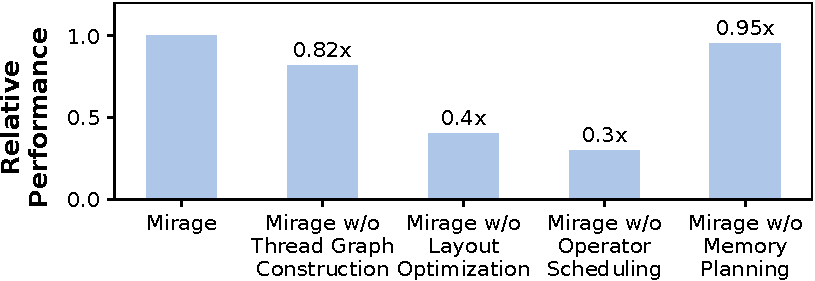
\includegraphics[width=\columnwidth]{figs/ablation-crop.pdf}
    \vspace{\captionvspace}
    \caption{Ablation study on optimizations used in Mirage. We evaluate the performance degradation when disabling each optimization independently. The evaluation is performed on A100 for GQA with batch size $1$.}
    \vspace{\captionvspace}
    \label{fig:ablation-optimization}
\end{figure}

We conduct an ablation study to evaluate the impact of thread graph construction and optimizations introduced in \S\ref{sec:optimizer}, including layout optimization, operator scheduling, and memory planning. Specifically, we measure the performance degradation of the best \graph discovered by \sys when each optimization is disabled independently. The study is conducted on an A100 using the GQA benchmark with a batch size of $1$. The results, shown in \Cref{fig:ablation-optimization}, indicate that disabling any individual optimization leads to a performance degradation ranging from $5\%$ to $70\%$.
